% !TEX root = mythesis.tex

%------------------------------------------------------------------------------
\chapter{Zusätzliche Graphen}
\label{sec:graphs}
%------------------------------------------------------------------------------

\begin{figure}[htbp]
    \label{fig:beta23a}
    \centering
    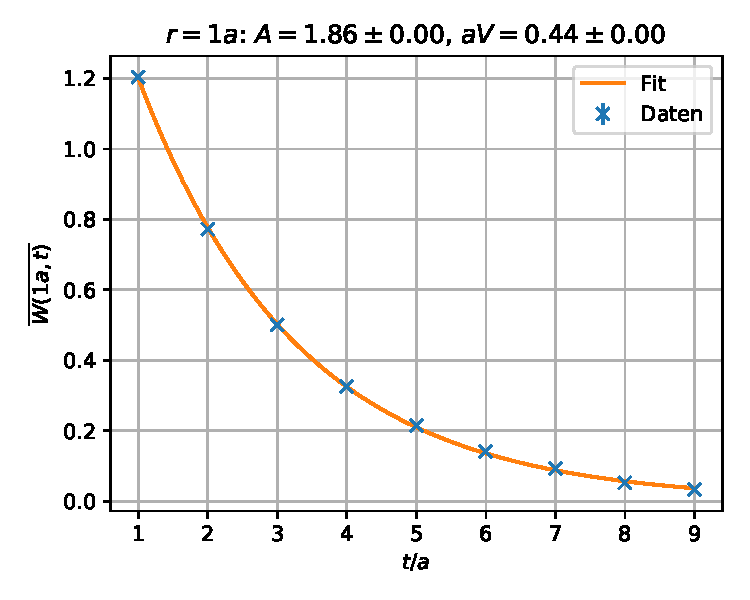
\includegraphics[width=.45\textwidth]{loopResultsBeta23r1}
    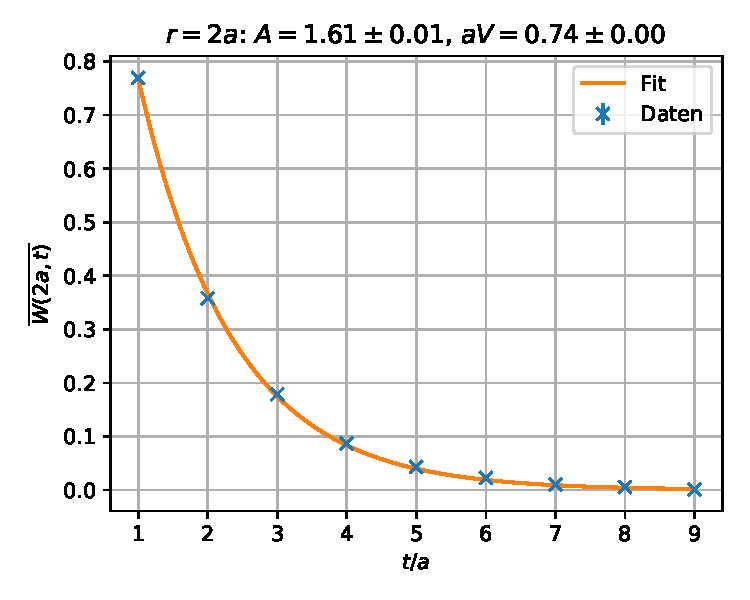
\includegraphics[width=.45\textwidth]{loopResultsBeta23r2}
    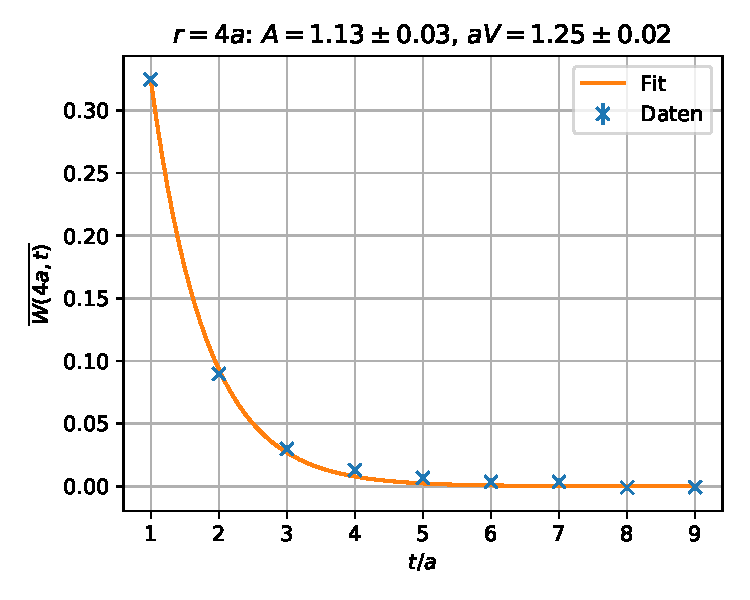
\includegraphics[width=.45\textwidth]{loopResultsBeta23r4}
    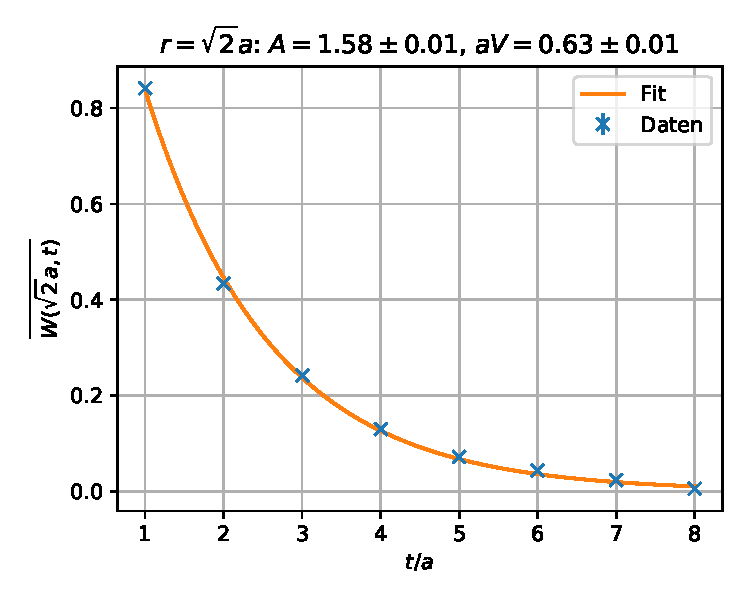
\includegraphics[width=.45\textwidth]{loopResultsBeta23rSqrt2}
    \caption{Messwerte der Wilson-Loops bei $\beta=2.3$ und festegehaltenem
    $r$. Verwendetes Modell: $\overline{W(r,t)} = A \cdot \exp(-aV(r) t/a)$.}
\end{figure}

\begin{figure}[htbp]
    \label{fig:beta23b}
    \centering
    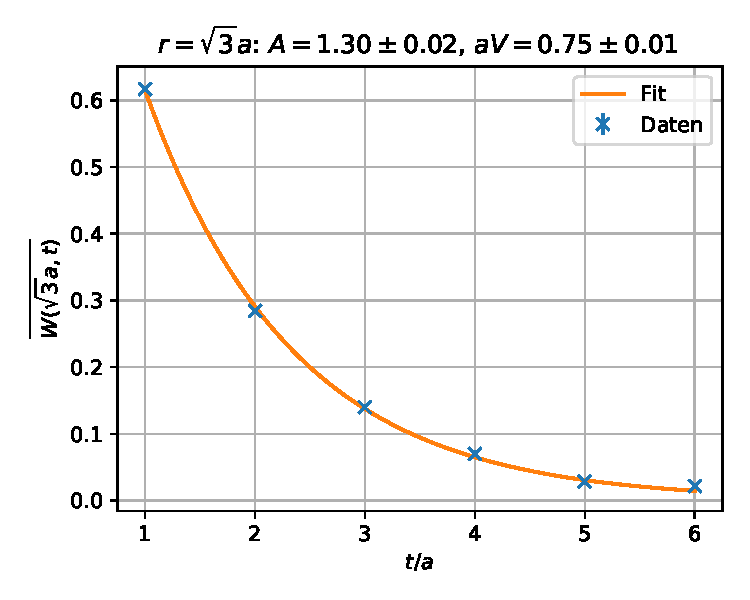
\includegraphics[width=.45\textwidth]{loopResultsBeta23rSqrt3}
    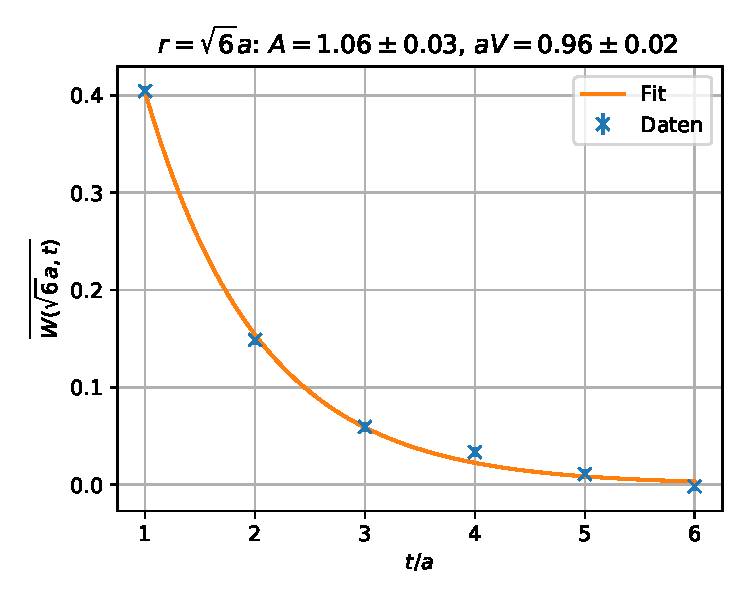
\includegraphics[width=.45\textwidth]{loopResultsBeta23rSqrt6}
    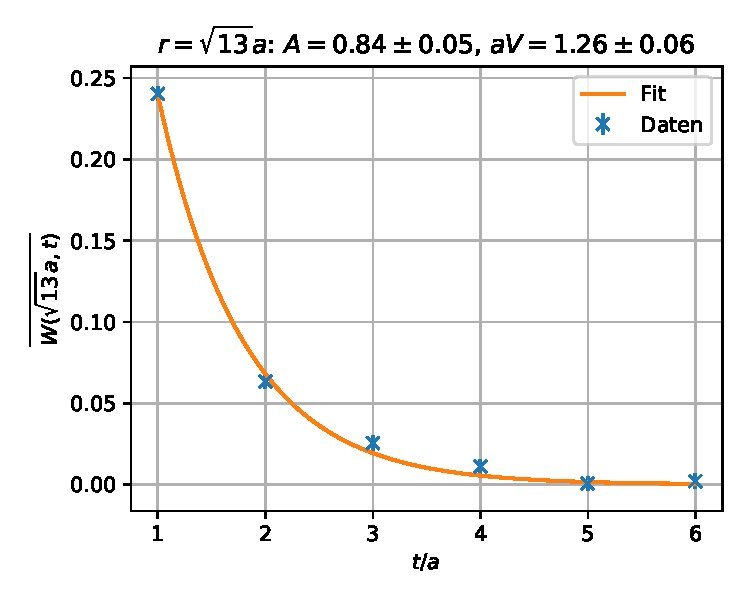
\includegraphics[width=.45\textwidth]{loopResultsBeta23rSqrt13}
    \caption{Messwerte der Wilson-Loops bei $\beta=2.3$ und festegehaltenem
    $r$. Verwendetes Modell: $\overline{W(r,t)} = A \cdot \exp(-aV(r) t/a)$.}
\end{figure}
